\documentclass[11pt,twocolumn]{article} 

\usepackage[spanish]{babel}
\usepackage{url, hyperref}
\usepackage{tabularx}
\usepackage{graphicx}
\DeclareGraphicsExtensions{.png}
\title{
\vspace{-3cm}   
Sistemas de Autentificaci\'on
}

\author{ 
Jorge Rubens Lipa Challapa\\
Edgar Jose Valencia Cayetano\\
Ronald Heredia Camacho\\
Fernando Soliz Tapia\\
\\
Universidad Mayor de San Sim\'on \\
Sociedad Cientifica de Estudiantes de Sistemas Inform\'atica\\
\url {http://www.scesi.org/}
}

\date{}

\begin{document}
\maketitle

\begin{abstract} 
Los diversos sistemas de autentificacion estan destinados a ofrece un control de acceso sobre un grupo determinado de personas y ofrecer datos estadísticos referentes a las entradas y salidas del personal que a su vez se interpretara como informaci\'on muy valiosa al momento de realizar seguimiento, frecuencia de accesos controlando los permisos de acceso al ambiente.  Pudiendo ser utilizado en diferentes \'areas de la industria donde se tenga que otorgar identificaciones \'unicas a un personal autorizado\\
\end{abstract}

\begin{abstract} 

\end{abstract}


\section{Introducci\'on}
Uno de los problemas de seguridad mas frecuentes, en estos tiempos, a sido el control de acceso a ambientes que requieren de una identificaci\'on. Ya sea por la cantidad de usuarios o tama\~no del ambiente. Las diferentes soluciones existentes llegan a tener dificultades, ya sea por tiempo, costo, personal encargado donde la implementaci\'on llega a ser laboriosa y compleja para los encargados. \\

Los sistema de autentificacion basados en RFID, permitir\'an, el manejo y control de personal y seguimiento de actividades a todo usuario que necesite una verificaci\'on de identidad utilizando tecnolog\'ias como \textit{Android, Arduino y Servicios web} estos permitir\'an elaborar instrumentos de control de acceso para el personal de una manera r\'apida y simple a un costo reducido.\\

\section{Antecedentes}

Generalmente se ve muy a menudo que todos los ambientes  con un nivel de acceso tengan una seguridad de acuerdo a un est\'andar ya establecido, para dar cierta privacidad y confidencialidad, esto puede variar ya que los dispositivos de acceso pueden o no hacer un seguimiento de las actividades sobre el personal. Esto deja al descubierto agujeros de seguridad en el ambiente que mas tarde se interpretara como debilidades y falencias de la instituci\'on.\\

La  informaci\'on  que proporcionaran estos dispositivos de acceso puede llegar a ser muy \'utiles, haciendo un seguimiento de las actividades del individuo o de un grupo de personas, de tal forma  que se tome decisiones con respecto a la informaci\'on obtenida.\\
 

Para asegurar la confidencialidad y privacidad, de ambientes que requieran un control de acceso limitando a un grupo de personas, se llega a la conclusi\'on: Que esta personas  requieren de permisos especiales, en este caso roles de acceso, para ingresar o realizar actividades que est\'en limitadas por un dispositivo de control. \\

\section{RFID}

RFID, Radio Frequency Identification permite transmitir la identidad de un objeto a una frecuencia con que se comunica con un dispositivo que reconoce al objeto. Este comportamiento esta basado en el modelo emisor receptor. \\

\begin{figure}[t]
  \begin{center}
    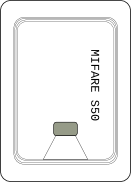
\includegraphics[width=2in]{mifare.png}
  \end{center}

  \caption{\small Dise\~no interno de Mifare S50.}
  \label{fig-label}
\end{figure}

\section{Mifare S50}

La tarjeta plástica PVC laminada tamaño ISO estándar: 85,7 x 54 x 0,82 mm, 6gr. aprox, trabaja a una frecuencia: 13,56 MHz integrado a un Chip Mifare de lectura y escritura la velocidad de transferencia para la lectura y escritura esta establecida a unos 106 Kbits/s. Esta tarjetas como sus predecesoras viene  con 1Kbytes de memoria EEPROM, de los cuales estan disponibles en 16 sectores y asignados con un numero de serie unico de 4 bytes\\
\\
La distancia maxima para realizar una lectura o escritura es de 10 cm, los datos pueden permanecer almacenados por al menos 10 a\~nos. \\
\\
Tal como se muestra en la Figura 1. El esquema de la tarjeta esta dividido en dos partes:\\

\begin{itemize}
	\item Antena de a cobre
	\item Chip Mifare.
\end{itemize}

La funcionalidad de esta tarjeta varia en funcionalidad, como ser para autentificaci\'on, y monetizaci\'on. En la actualidad varias ciudades emplean de diferentes formas el uso de los dispositivos de identificicaci\'on, como venta de pasajes para autobuses, identificacion en tarjetas de credito, credenciales medicas. inventarios de productos y ganado. 


\section{Aporte tecnol\'ogico}

La implementaci\'on de hardware libres como Arduino impulsara la adopci\'on de los dispositivos electr\'onicos en otras \'areas gracias a la gran variedad de m\'odulos que cuenta y tambi\'en tecnolog\'ias como los servicios web que descentralizaran la informaci\'on y el monitoreo en tiempo real, permitiendo a diferentes dispositivos tener informaci\'on de manera inmediata mediante celulares, tablets, paginas web.\\



Para ello tenemos los proyectos Centinela y  ..  tiene pensado facilitar tanto las transacciones de dinero como autentificacion de persona.

\section{Proyecto Centinela}

Centinela, Control y seguimiento de actividades de acceso para la identificaci\'on de personal. Basado en tecnolog\'ias  open source. Dicho sistema  proveera el acceso a ambientes controlados mediante RFID, los datos ser\'an mandados mediante un servicio web para su procesamiento en un servidor. Figura 2.\\

Los datos obtenidos se utilizaran para realizar reportes de seguimiento a los usuarios registrados. Los dispositivos de recolecci\'on estan basados en dise\~no construidos con arduino, compatibles con dispositivos m\'oviles que tengan NFC y lectores de alta frecuencia (UHF).\\

Cabe resaltar que cada uno de estos dispositivos de trabaja de manejar distinta y su uso variar de acuerdo al usuario.\\

\begin{figure}[!h]
  \begin{center}
    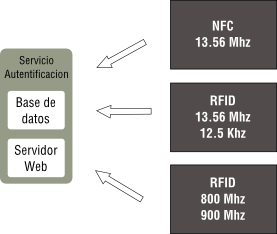
\includegraphics[width=2in]{architect.png}
  \end{center}

  \caption{\small Modelo de implementacion para el Proyecto Centinela.}
  \label{fig-label}
\end{figure}

\section{Proyecto Colectivo Virtual}

Orientado al registro y seguimiento de cr\'edito asignado a un dispositivo RFID, con la funcionalidad Wallet de las tarjetas Mifare S50. Con esto se tendra un registro del cambio de cantidad asignado a una identificaci\'on para que pueda ser utilizando en forma de pago o cambio, por ejemplo en un auto bus, pagar los pasajes con una identificaci\'on RFID, recargar cr\'editos en un vale de descuento, Monedero virtual y demas usos que tengar que ver con cambios de estado para un incremento y decremento.\\

Un dispositivo de control realizara la transacci\'on y guardara los cambios en el dispositivo de manera rapida. la recargar se hara mediante  otro dispositivo que guardara los datos de usuarios y la cantidad del incremento o decremento.



\section{Modelo de trabajo}  

Independientemente del proyecto, un sistema de autentificacion es necesario para administrar y gestionar la informacion de los usuarios y los dispositivos de control.

El m\'etodo de desarrollo comprende tres \'areas  que dar\'an como resultado a un sistema de autentificaci\'on  para los diferentes  proyecto citados.\\

	\subsection{ Sistema web }
	
	\begin{description}
		\item [Registro basado en roles] Gesti\'on de los usuarios como el administrador, seguridad y personal com\'un.
		\item [Dispositivos de control] Gesti\'on de los dispositivos de control.
		\item [Seguimiento] Seguimiento de las actividades referentes a las credenciales de autentificaci\'on.
		\item [Reportes de seguimiento] An\'alisis de datos referentes a las actividades de los usuarios autentificados.
	\end{description}
	
	\subsection{Aplicaci\'on m\'ovil}		
	
	 \begin{description}
		 \item[Seguimiento de actividad] Seguimiento de procesos de identificaci\'on a los dispositivos de control.
		 \item[Reporte personal] Reporte de seguimiento de actividad personal.
	 \end{description}
	
	\subsection{Dispositivo electr\'onico}
	
	 \begin{description}
		 \item[Comunicaci\'on con sistema web] Interfaz de acceso al sistema web mediante una conexi\'on Ethernet.
		 \item[Verificaci\'on de identidad] Control de acceso mediante RFID.
		 \item[Interaccion con usuario] Estado de verificaci\'on mediante componentes electr\'onicos.
	 \end{description}			

\section{Desarrollo}

Para la realizaci\'on del proyecto \textit{Centinela}, se a clasificado las herramientas que servir\'an para la culminaci\'on del prototipo inicial, establecidos en las secciones: Componentes electr\'onicos, Herramientas de prueba, Herramientas de desarrollo.

	\subsection{Componentes electr\'onicos}

	Los  dispositivos electr\'onicos que se mencionaran estan limitados en base al prototipo que se pretende realizar:\\
	
	\begin{enumerate}
		\item Arduino Uno
		\item Tarjeta RFID Mifare S50
		\item Lector RFID RS232 13.56 Mhz
		\item Modulo de red (arduino) ENC28J60
		\item Modulo SD Card (arduino)
	\end{enumerate}
	
	\subsection{Equipamiento}

	Para establecer la funcionalidad del sistema se requiere equipos que soportes las tecnolog\'ias de desarrollo, para esto se ha determinado los componente a continuaci\'on: \\
	
	\begin{enumerate}
		\item Raspberry Pi Modelo B 
		\item Router inalambrico y red
		\item Cableado de red 
		\item Tableta o m\'ovil para el acceso al sistema
	\end{enumerate}
	
	\subsection{Herramientas de desarrollo}
	
	Esta secci\'on detalla el software que se utilizara para el desarrollo en todos los ambientes de trabajo del proyecto Centinela ,detallando su descripci\'on con la versi\'on y su desempe\~no segun :
	
	\begin{enumerate}
		\item Apache v2.2
		\item PHP v5.4
		\item PostgreSQL v9.3
		\item Laravel Framework v4.2
		\item Android v4.0.4
		\item Arduino IDE v1.0.5
	\end{enumerate}

\section{Conclusiones y recomendaciones}
Como se pudo apreciar con esta combinaci\'on de tecnolog\'ias y se puede decir que la adopci\'on de RFID de la mano de Arduino es muy aceptable seg\'un nuestra experiencia ya que los  aspectos t\'ecnicos ya quedan relevados a los m\'odulos que disponen dejando la programaci\'on de estos a nuestro criterio donde se puede apreciar el conocimiento que se obtuvo ya que esta nos compete al ser la rama troncal de nuestra facultad. \\
	
Aclarar que este tipo de sistema esta dispuesto de forma general y planeado para ser implementado primeramente en ambientes donde requieran identificaci\'on como en conferencia, seminarios, laboratorios. La disponibilidad de los dispositivos hace que su implementaci\'on llegue a una escala aun mayor a las ya mencionadas.
\section{Bibliograf\'ia}
	
	\begin{itemize}
		\item  Tedjasaputra, Adi (18 de diciembre 2006). «RFID Tag Attachments». RFID Asia. Consultado el 3 de agosto 2007.
		\item Dargan, Gaurav; Johnson,Brian; Panchalingam, Mukunthan; Stratis, Chris (2004), The Use of Radio Frequency Identification as a Replacement for Traditional Barcoding
		
		\item "REST APIs must be hypertext driven by Roy Fielding". Roy.gbiv.com. 2008-10-20. Retrieved 2013-02-07.
	\end{itemize}
	
\end{document}          